\documentclass{article}
\input{C:/Users/aryay/OneDrive/Shared Files/Programs/Preamble.tex}


\title{Geodesics on a Cone}
\author{Arya Yae}
\date{}

\begin{document}

\begin{center}
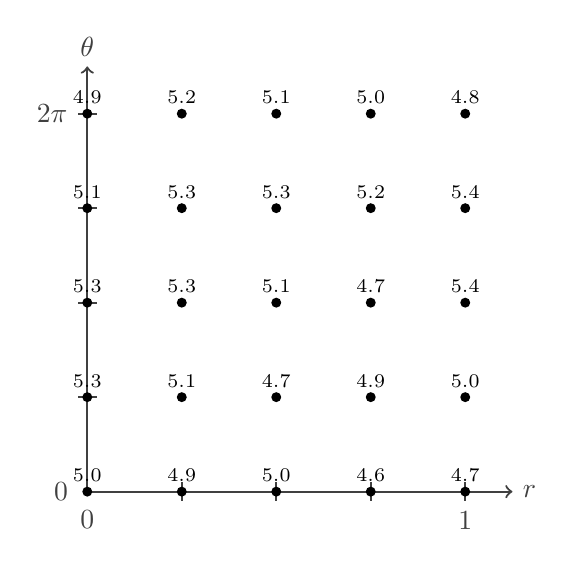
\begin{tikzpicture}[scale=1.2]
    % Axes
    \draw[darkgray, thick, ->] (0,0) -- (4.5,0) node[right] {$r$};
    \draw[darkgray, thick, ->] (0,0) -- (0,4.5) node[above] {$\theta$};

    % Tick marks
    \node[left, text=darkgray] at (-0.1,0) {$0$};
    \node[below, text=darkgray] at (0,-0.1) {$0$};
    \foreach \x in {1, 2, 3} {
        \draw[darkgray, thick] (\x, 0.1) -- (\x, -0.1);
    }
    \draw[darkgray, thick] (4, 0.1) -- (4, -0.1) node[below, text=darkgray] {$1$};

    \foreach \y in {1, 2, 3} {
        \draw[darkgray, thick] (0.1, \y) -- (-0.1, \y);
    }
    \draw[darkgray, thick] (0.1, 4) -- (-0.1, 4) node[left, text=darkgray] {$2\pi$};

    % Lattice points
    \foreach \x in {0, 1, ..., 4} {
        \foreach \y in {0, 1, ..., 4} {
            \pgfmathsetmacro{\randval}{5.0 + 0.4*rand}
            \fill[black] (\x, \y) circle (1.5pt) node[above, font=\scriptsize] {\pgfmathprintnumber[fixed, precision=1, fixed zerofill]{\randval}};
        }
    }
\end{tikzpicture}
\end{center}

\end{document}